\chapter*{07.08. --- Wieloryby! Wieloryby?!}

Z samego rana poszliśmy na spacer na otaczające dolinę klify --- głów\-ną \href{http://www.visithusavik.com/attractions/asbyrgi-canyon/}{atrakcję} okolicy. Żadnych trudności terenowych, niewielki dystans, pogoda (jeszcze) w miarę stabilna. Ot, taka przechadzka na rozprostowanie nóg.

Na śniadanie po raz pierwszy zjedliśmy (łącznie, na grupę): 1~kg paszy zalanej 1~l mleka i 1~l surmjolka\footnote{Islandzki \emph{súrmjólk} to po prostu kwaśne mleko.} --- czyli średnio po 2000~kilokalorii na osobę! (Należy w tym miejscu zaznaczyć, że zaczynaliśmy od połowy tej porcji, a i tak ledwie taką ilość przejadaliśmy --- teraz te kilogramy to tak akurat na styk.)

\img{./photos/x-s-2014-08-07_10-26-01__82.jpg}{asbyrgi_camping}{Nocleg u stup klifów.}
\img{./photos/x-s-2014-08-07_15-19-08__209.jpg}{asbyrgi_breaking_the_law}{Znów łamiemy prawo \sad}

Z Ásbyrgi wyruszamy przy wietrze w plecy --- szok i niedowierzanie! Radość trwa krótko, bo po 25~km, gdy tylko zatrzymaliśmy się na posiłek, zaczęło padać.

\medskip

Coś na rozluźnienie. Scenka wydarzyła się na koniec solidnego podjazdu. Ledwo zipiemy, pot się leje, wieje nam w mordę. \newline
--- No i co tak ludzie nam zdjęcia robią? --- spytałem. --- Nawet się nie uśmiechną! Dobrego słowa nie powiedzą! A do tego mają tylko ten znudzony wyraz twarzy\textellipsis \newline
--- Eee\textellipsis dobrze że robią\textellipsis --- odparł Put. \newline
--- No to niech chociaż jakieś ciastko w zamian dadzą! --- stwierdziłem. \newline
Na to Put, z szerokim uśmiechem: \newline
--- Czyli chciałbyś być taką dziwką rowerową? Sprzedawałbyś swoje podjazdy za ciastka?

\section*{Húsavík}

Specjalnie zajechaliśmy odpowiednio wcześniej do Húsavíku, by Put i Kasia mogli załapać się na \emph{whale watching}\footnote{Oglądanie wielorybów to główna atrakcja północno-wschodniej części Islandii.}. Mimo intensywnej agitacji ze strony Puta, ani Karolina ani ja nie zdecydowaliśmy się na dołączenie. Powody? Karolina widziała już z bliska delfiny (a~to prawie jak widzieć wieloryby), gdy pływała żaglówką po Morzu Północnym, mnie natomiast do rejsu nie zachęcała pogoda (zimno, pochmurno, wietrznie). Co więcej, żadnej gwarancji zobaczenia wieloryba nie ma --- pani w informacji powiedziała, że dwa poranne rejsy nic nie widziały, a kolejny był już ciut lepszy, lecz też bez szału. \emph{,,Natomiast na pewno mogę zagwarantować, że będzie chłodno!''} --- dodała z uśmiechem. (Dla ustalenia uwagi, rejs trwa około trzy godziny).

Ja i Karolina pożegnaliśmy więc ,,wielorybników'' i pojechaliśmy zakładać obozowisko. Kemping kosztował 1200~kr za osobę (prysznic płatny dodatkowo 500~kr); był wyposażony w suszarnię z prawdziwego zdarzenia i małą kuchnię turystyczną z paroma palnikami i~paroma stołkami. Gdy już się rozgościliśmy i przebraliśmy, ruszyliśmy na miasto ,,na rybę'' --- to znaczy głównie chodziło nam o to, by po ponad dwóch tygodniach tułaczki wreszcie zjeść coś normalnego.

Po obejściu wszystkich (czterech) portowych knajp i wnikliwym porównaniu menu oraz cen wybraliśmy restaurację \href{https://www.facebook.com/naustid}{Naustið}. Musieliśmy dobrą chwilę czekać na wolny stolik (taki był ruch), lecz przynajmniej wreszcie czekaliśmy na coś stojąc w ciepłym pomieszczeniu! Zamówiliśmy zupę rybną oraz \emph{,,2x szaszłyk rybny na 1 talerzu''} --- coś pysznego! W zupie pływała duża ilość tłuściutkich krewetek, a całość była dobrze doprawiona. Szaszłyczane rybie mięso było bardzo delikatne, a w ramach przybrania występowały: małe ziemniaczki, sałata, feta\textellipsis Ach, to było jak podróż do innego, lepszego świata! Za oknem siąpi i hula wiatr, a my grzejemy się, siedząc przy stoliku tuż obok kaloryfera i zajadamy się takimi smakołykami\textellipsis I tylko żal było się tak szybko zmywać (bo ani się oglądnęliśmy, a zrobiła się 22:00 --- godzina zamykania lokalu).

W drodze powrotnej zahaczyliśmy jeszcze o grill-bar przy stacji benzynowej (nie, bynajmniej nie po to, by psuć sobie smak, tylko żeby rozmienić pieniądze) i\textellipsis to było coś koszmarnego. To było traumatyczne wręcz doświadczenie --- wejście do takiego czegoś po wizycie w przytulnej knajpce. Wejście do miejsca, gdzie przy trupim świetle świetlówek zmarnowani ludzie męczą hamburgery i frytki. Brr\textellipsis

%TODO: zdjęcie posiłku w barze rybnym

Cóż, i tak mimo wszystko trochę zepsuliśmy sobie smak szaszłyków i zupy rybnej, bo droga powrotna na kemping tak nas zmęczyła, że konieczne było dojedzenie chlebem z~szoko\textellipsis

Wielorybnicy wrócili o 23:30, nie zobaczywszy ani jednej ,,taakiej'' ryby. Na pocieszenie wrzucili za to na fb swoje sweet-selfie-focie w gustownych sztormiakach zawodowego rybaka morskiego \wink

PS. Dziś na podjazdach Kasia pokazała pełną klasę i prawdziwego ducha walki --- gratulacje!

%TODO: zrobić z tego środowisko
%\img{./photos/x-s-2014-08-07_19-54-58__84.jpg}{whalewatching_clothing}{Kasia w pełnym rynsztunku}

\begin{figure}[h]
	\centering
	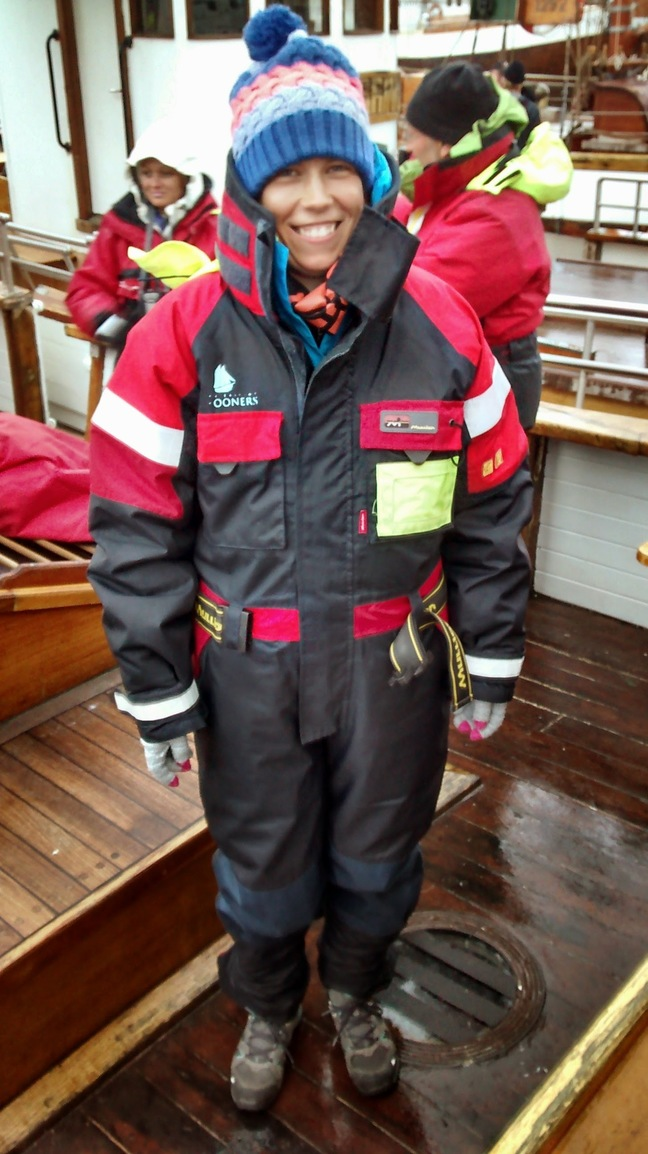
\includegraphics[height=.8\linewidth]{./photos/x-s-2014-08-07_19-54-58__84.jpg}
	\caption*{Kasia w pełnym rynsztunku}
	\label{img:whalewatching_clothing}
\end{figure}

\pagebreak
